%%%%%%%%%%%%%%%%%%%%%%
% NASTAVENÍ FEKT.TEX %
%%%%%%%%%%%%%%%%%%%%%%

% Pokud následující řádky zakomentujete, na titulní straně se nezobrazí.

% Nadpis dokumentu (kód předmětu)
\newcommand{\name}{Documentation}
% Podnadpis dokumentu (název předmětu)
\newcommand{\subname}{Sensitive file sharing application} 
% Seznam autorů
\newcommand{\authors}{Martin Bezecný, Karel Ramiš, Marek Szymutko, Adam Tuček}
% Seznam korektorů
%\newcommand{\corrections}{}
% Popis dokumentu
%\newcommand{\docdesc}{}
% Zařazení dokumentu (studijní program)
% \newcommand{\docgroup}{Informační bezpečnost, FEKT VUT}
% Odkaz
% \newcommand{\docurl}{https://github.com/VUT-FEKT-IBE/FEKT.tex}

% Přepsáním argumentu na 'true' zapnete balíček 'minted' pro sázení kódu.
% Pro jeho použití lokálně musíte mít v systému dostupný Python 3, python
% knihovnu 'minted' a PDFLaTeX musíte spouštět s argumentem '-shell-escape'.
% Místo něj můžete použít prostředí 'lstlisting'.
\newcommand{\docminted}{false}


%%%%%%%%%%%%%%%%%%%%
% OBECNÉ NASTAVENÍ %
%%%%%%%%%%%%%%%%%%%%

\newcommand{\fekttexversion}{2.0}

\documentclass[
    % Velikost základního písma je 12 bodů
    12pt,
    % Formát papíru je A4
    a4paper,
    % Oboustranný tisk
    twoside,
    % Záložky a metainformace ve výsledném PDF budou v kódování unicode
    unicode,
]{article}

% Kódování zdrojových souborů
\usepackage[utf8]{inputenc}
% Kódování výstupního souboru
\usepackage[T1]{fontenc}

% Geometrie stránky
\usepackage[
    % Horní a dolní okraj
    tmargin=25mm,
    bmargin=25mm,
    % Vnitřní a vnější okraj
    lmargin=30mm,
    rmargin=20mm,
    % Velikost zápatí
    footskip=17mm,
    % Vypnutí záhlaví
    nohead,
]{geometry}

% Zajištění kopírovatelnosti a prohledávanosti vytvořených PDF
\usepackage{cmap}
% Podmínky (pro použití v titulní straně)
\usepackage{ifthen}

%%%%%%%%%%%%%%%
% FORMÁTOVÁNÍ %
%%%%%%%%%%%%%%%

% Nastavení stylu nadpisů
\usepackage{sectsty}
% Formátování obsahů
\usepackage{tocloft}
\setcounter{tocdepth}{1}
% Odstranění mezer mezi řádky v seznamech
\usepackage{enumitem}
\setlist{nosep}
\setitemize{leftmargin=1em}
\setenumerate{leftmargin=1.5em}
\renewcommand{\labelitemi}{--}
\renewcommand{\labelitemii}{$\circ$}
\renewcommand{\labelitemiii}{$\cdot$}
\renewcommand{\labelitemiv}{--}
% Sázení správných uvozovek pomocí '\enquote{}'
\usepackage{csquotes}
% Vynucení umístění poznámek pod čarou vespod stránky
\usepackage[bottom]{footmisc}
% Automatické zarovnání textu k předcházení vdov a parchantů
\usepackage[defaultlines=3,all=true]{nowidow}
% Zalomení části textu pokud není na současné stránce dost místa
\usepackage{needspace}
% Nastavení řádkování
\usepackage{setspace}
\onehalfspacing
% Změna odsazení odstavců
\setlength{\parskip}{1em}
\setlength{\parindent}{0em}

% Bezpatkové sázení nadpisů
\allsectionsfont{\sffamily}
% Změna formátování nadpisu a podnadpisů v Obsahu
\renewcommand{\cfttoctitlefont}{\Large\bfseries\sffamily}
\renewcommand{\cftsubsecdotsep}{\cftdotsep}

% Použití moderní/aktualizované sady písem
\usepackage{lmodern}

%%%%%%%%%%%
% NADPISY %
%%%%%%%%%%%

\usepackage{titlesec}

\titlespacing*{\section}{0pt}{10pt}{-0.2\baselineskip}
\titlespacing*{\subsection}{0pt}{0.2\baselineskip}{-0.2\baselineskip}
\titlespacing*{\subsubsection}{0pt}{0.2\baselineskip}{-0.2\baselineskip}
\titlespacing*{\paragraph}{0pt}{0pt}{1em}

%%%%%%%%%%
% ODKAZY %
%%%%%%%%%%

% Tvorba hypertextových odkazů
\usepackage[
    breaklinks=true,
    hypertexnames=false,
]{hyperref}
% Nastavení barvení odkazů
\hypersetup{
    colorlinks,
    citecolor=black,
    filecolor=black,
    linkcolor=black,
    urlcolor=blue
}

%%%%%%%%%%%%%%%%%%%%%%%%%%%
% OBRÁZKY, GRAFY, TABULKY %
%%%%%%%%%%%%%%%%%%%%%%%%%%%

% Vkládání obrázků
\usepackage{graphicx}
\usepackage{subfig}
% Nastavení popisů obrázků, výpisů a tabulek
\usepackage{caption}
\captionsetup{justification=centering}
% Grafy a vektorové obrázky
\usepackage{tikz}
\usetikzlibrary{shapes,arrows}
% Složitější tabulky
\usepackage{tabularx}
\usepackage{multicol}

% Sázení osamocených float prostředí v horní části stránky
\makeatletter
\setlength{\@fptop}{0pt plus 10pt minus 0pt}
\makeatother

% Vynucení vypsání floating prostředí pomocí \FloatBarrier
\usepackage{placeins}

% Rámečky
\usepackage{mdframed}

%%%%%%%%%%%%%%
% MATEMATIKA %
%%%%%%%%%%%%%%

% Sázení matematiky a matematických symbolů ('\mathbb{}')
\usepackage{amsmath}
\usepackage{amssymb}
% Sázení fyzikálních veličin
\usepackage{siunitx}

%%%%%%%%%%%%%%%%%
% ZDROJOVÉ KÓDY %
%%%%%%%%%%%%%%%%%

% Sazba zdrojových kódů
\usepackage[formats]{listings}
% Přepnutí prostředí 'code' do režimu výpisu kódu
\newenvironment{code}{\captionsetup{type=listing}}{}

\lstset{
    basicstyle=\small\ttfamily,
    numbers=left,
    numberstyle=\tiny,
    tabsize=4,
    columns=fixed,
    showstringspaces=false,
    showtabs=false,
    keepspaces,
}

% Balíček 'minted' budeme používat pouze pokud je jeho hodnota nastavena na 'true'
\providecommand{\docminted}{false}
\ifthenelse{\equal{\docminted}{true}}
{
    % Sazba zdrojových kódů
    \usepackage[newfloat]{minted}
    % Nastavení barev 'minted' kódů
    \usemintedstyle{pastie}
}
{
    % \docminted není 'true', nic neprovádíme
    % Pokud je v dokumentu 'minted' prostředí, dokument se nepodaří přeložit.
}

%%%%%%%%%%%%%%%%%%%
% VLASTNÍ PŘÍKAZY %
%%%%%%%%%%%%%%%%%%%

\newcounter{todo}
\newcommand{\TODO}[1]{%
    \addtocounter{todo}{1}%
    \textcolor{red}{%
    \textbf{\sffamily\small{TODO \thetodo}%
    \ifthenelse{\equal{#1}{}}{}{:}%
    } %
    #1%
    }%
}

%%%%%%%%%%%
% TITULKA %
%%%%%%%%%%%

\newcommand{\titulka}{
    \vspace*{2em}
    \begin{center}
        \ifthenelse{\isundefined{\name}}{}{{\Huge \bfseries \name{}}}

        \ifthenelse{\isundefined{\subname}}{}{{\huge \bfseries \subname{}}}

        \vspace*{2em}

        \ifthenelse{\isundefined{\docdesc}}{}{{\Large \docdesc}}

        \vspace*{1em}

        \ifthenelse{\isundefined{\docgroup}}{}{\docgroup}

        \ifthenelse{\isundefined{\docurl}}{}{\url{\docurl}}
    \end{center}

    \vfill

    \ifthenelse{\isundefined{\authors}}{}{\authors{}}
    \ifthenelse{\isundefined{\corrections}}{}{\\\small (korektury \corrections{})}


    \thispagestyle{empty}
    \newpage
}

%%%%%%%%%%%%
% DOKUMENT %
%%%%%%%%%%%%

\begin{document}

\titulka{}

\tableofcontents
\thispagestyle{empty}

\setcounter{page}{0}

\section{Installation}

Installation is done using the following steps for RPM based system. For APT based systems, replace \texttt{dnf} with \texttt{apt}. 
\begin{lstlisting}[language=bash]
    sudo dnf install python3 python3-pip python3-virtualenv
    python3 -m venv .venv
    source .venv/bin/activate
    python3 -m pip install pdm
    pdm install
\end{lstlisting}

For running the application you can use the following command:
\begin{lstlisting}[language=bash]
    python3 main.py
\end{lstlisting}

\section{GUI}
The GUI start by running `python3 main.py` in the virtual enviroment.

\subsection{Login screen}

\subsection{Main window}

\subsubsection{File selection}

\subsubsection{Friend addition}

\subsubsection{Listing of users}

\subsubsection{Listing queued files}

\subsubsection{Friend selection}

\subsubsection{File sharing}
\section{Functionality description}
This section goes over the app functionalities and how they are designed and implemented.

\subsection{Login}
This is a section going over logging in to the application. If it is the first time the user uses the application they will have to create an account with username
and password. Otherwise only password is required. If user inserts a password that does not match their corresponding password stored in database the 
"Invalid password" message is displayed. If the password is correct, the main window of the application is shown.

This is implemented in the file \texttt{main.py} in the function \texttt{start\_app()}.

\subsection{File selection}
Selecting files is handled by the button \texttt{Choose a file to be sent}. When the button is pressed, a dialog window is opened where the user can select
a file. The implementation of this is done using module \texttt{filedialog} from \texttt{tkinter} library. If a file is not selected, the window won't let them
select a path that is not pointing to a file. If the window is closed without selecting a file, the filepath is kept empty.

The code itself can be seen in file \texttt{file\_share/app/app.py} in the function \texttt{get\_file()}.

\subsection{Listing users}
There are two functionalities that are related to listing users. The first one is listing all non-friend users that are in the database. The second one 
is listing all users that the user has added as friends. Both of these open new windows where the users are listed. The difference between these two windows
is that in the window where non-friend users are listed, there is a button to add them as a friend.

The list friends functionality is simpler and it is done by retrieving all users from the database and filtering out the ones that are friends with the user.
The method that handles this is the \texttt{get\_all\_users} from \texttt{file\_share/database/\_\_init.py\_\_}, where there is friend parameter which is by default set to \texttt{True}.\\
The non-friends is a bit more complicated. First, the list of all users except friends is collected from the database. It is listed in the window. If user wants 
to add a friend, they select that user from the list and press button "Befriend this user", this calls a function \texttt{befriend} in \texttt{file\_share/database/\_\_init.py\_\_}.
This adds the user as a friend by setting the \texttt{is\_friend} attribute to \texttt{True}.

\subsection{File sending initialization}
For this core functionality there is a flow chart attached for easier comprehensibility. It is implemented in function \texttt{send\_file} in \texttt{file\_share/app/app.py}.
The function first checks if the file for transfer is selected, if that is true, the file is then prepared for transfer and file transfer is attempted. Sending is done by 
function \texttt{send\_or\_store\_file} from \texttt{file\_share/sender/sender.py}. As a return there is a \texttt{SendStatus} object, which is enum created for this application.
There are 5 states that the object can be in, those can be viewed in \texttt{file\_share/definitions/enums.py}. Based on the state of the user which is passed to the function,
the file will either be sent, stored in outgoing queue or nothing will happen.\\

If the file is to be stored then it is scheduled to be added to files table in the database using \texttt{store\_file} from \texttt{file\_share/database/\_\_init.py\_\_}.

\begin{figure}[ht]
    \centering
    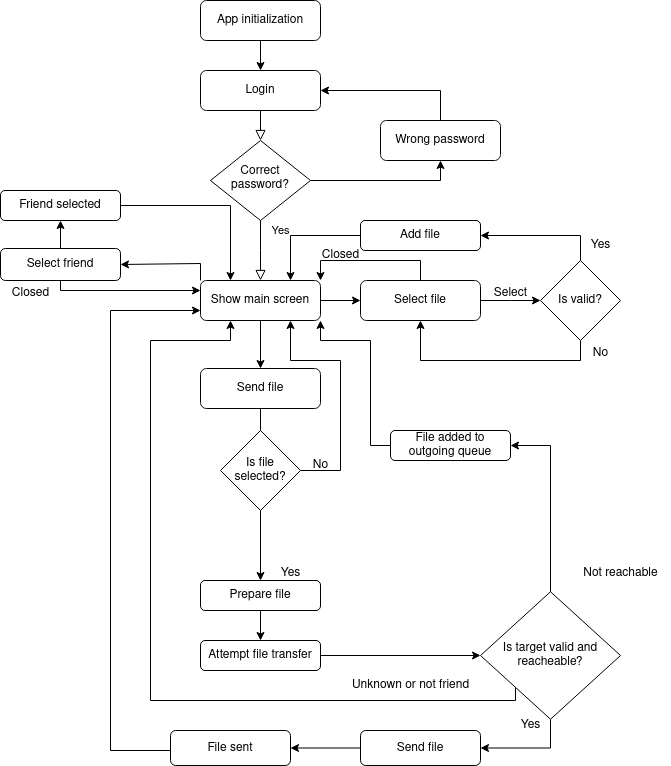
\includegraphics[scale = 0.5]{images/filesending.png}
    \caption{Flowchart of file sending initialization}
    \label{fig:flowchart}
\end{figure}
\subsection{File sending}
In this section the process of file transfer itself is described. It is accompanied by a figure that shows the sides of the communication and the steps
that each of the sides takes.\\
This whole process is based on using a one time use API key which is generated by the receiving side of the communication. This key is then used by the sender in 
the header of the file transfer as a verification of the communication. 
Firstly the sender extracts from the file object that is passed as a parameter the username of target user, then on the basis of this username retrieves the
address of this user from database, unless the file has address override in it. In which case the override address is used as a target address.\\
Then the SSL context of given username is taken and using aiohttp session a request is made to the target user. The target then verifies if the sender is a friend,
if not then exception 401 is raised and the communication is terminated by this exception. If the sender is a known friend, then an API key is generated, encoded using the senders public 
key extracted from their certificate and sent back to the sender as a response. This verification and key generating is done in \texttt{file\_share/receiver/receiver\_api.py} in method \texttt{auth()}.\\
When sender receives this API key, it is decrypted using the senders private key, then a FormData object is created, the file is added to it and finally a sending
is done with this FormData object, where the API key is included as the header.\\
On the receiving side, when the file transfer is done the API key is removed from database as it is one time use only. If the key is not found in database then
a 401 exception is raised and this ends the communication. Otherwise a new file object is created with the incoming attribute set to True, the object is timestamped,
and sender username is associated with it. Then it is added to the database table and the file's name is returned as a response.\\

\begin{figure}
    \centering
    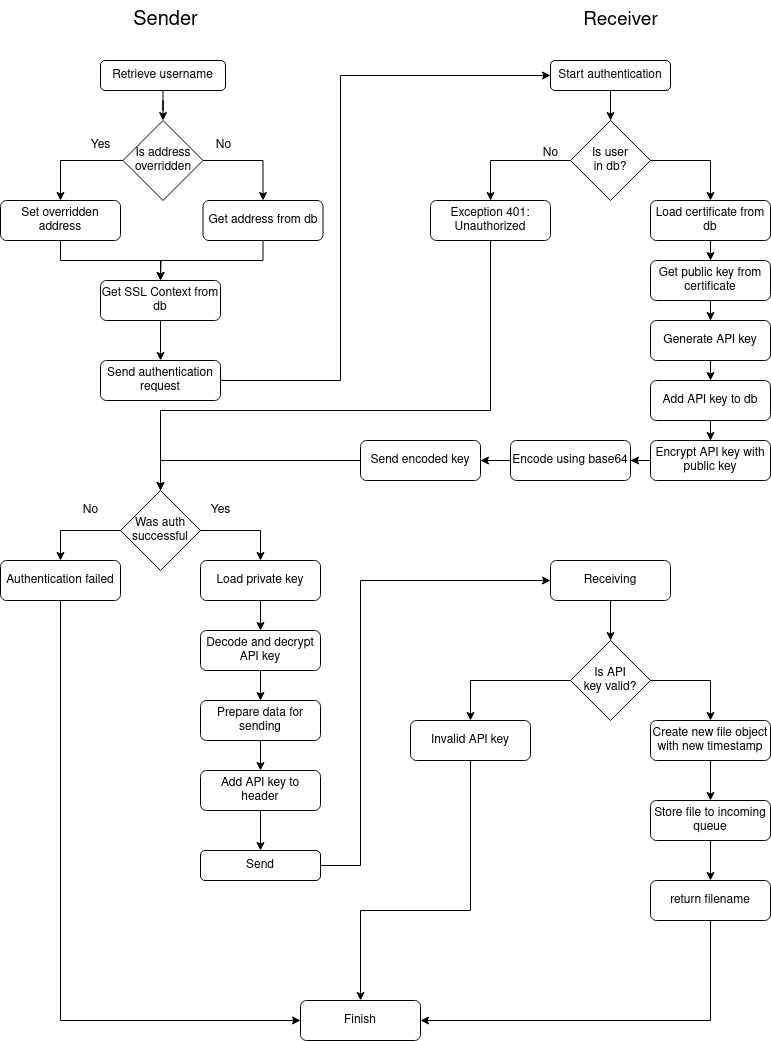
\includegraphics[scale = 0.5]{images/file_send.png}
    \caption{Flowchart of file transfer}
    \label{fig:filetransfer}
\end{figure}

\end{document}
